\label{sec:ablation_part1}

We shall do the following, details can be found in \texttt{ablation.ipynb}.
In brief, we perform \texttt{StandardScaler()} and \texttt{SMOTE} prior to the train/test split stage, as this would introduce data leakage to the train set, and in fact, significantly improve the results on the test set, though it falsely report models' performance.
We also realise that, either $(1000 \times 12)$ or $(12 \times 1000)$ can be flattened to $(12000,)$, the latter sounds more reasonable, as it places the lead axis before the time axis, and we hypothesize it would describe the raw ECG signals, more meaningfully and precisely.
However, we still keep the same established flattening order, i.e. $(1000 \times 12) \to (12000,)$.
Let us present the results obtained, by keeping the same configuration discussed earlier.

\begin{figure}[H]
    \caption{Comparison on class–wise precision for each model.}
    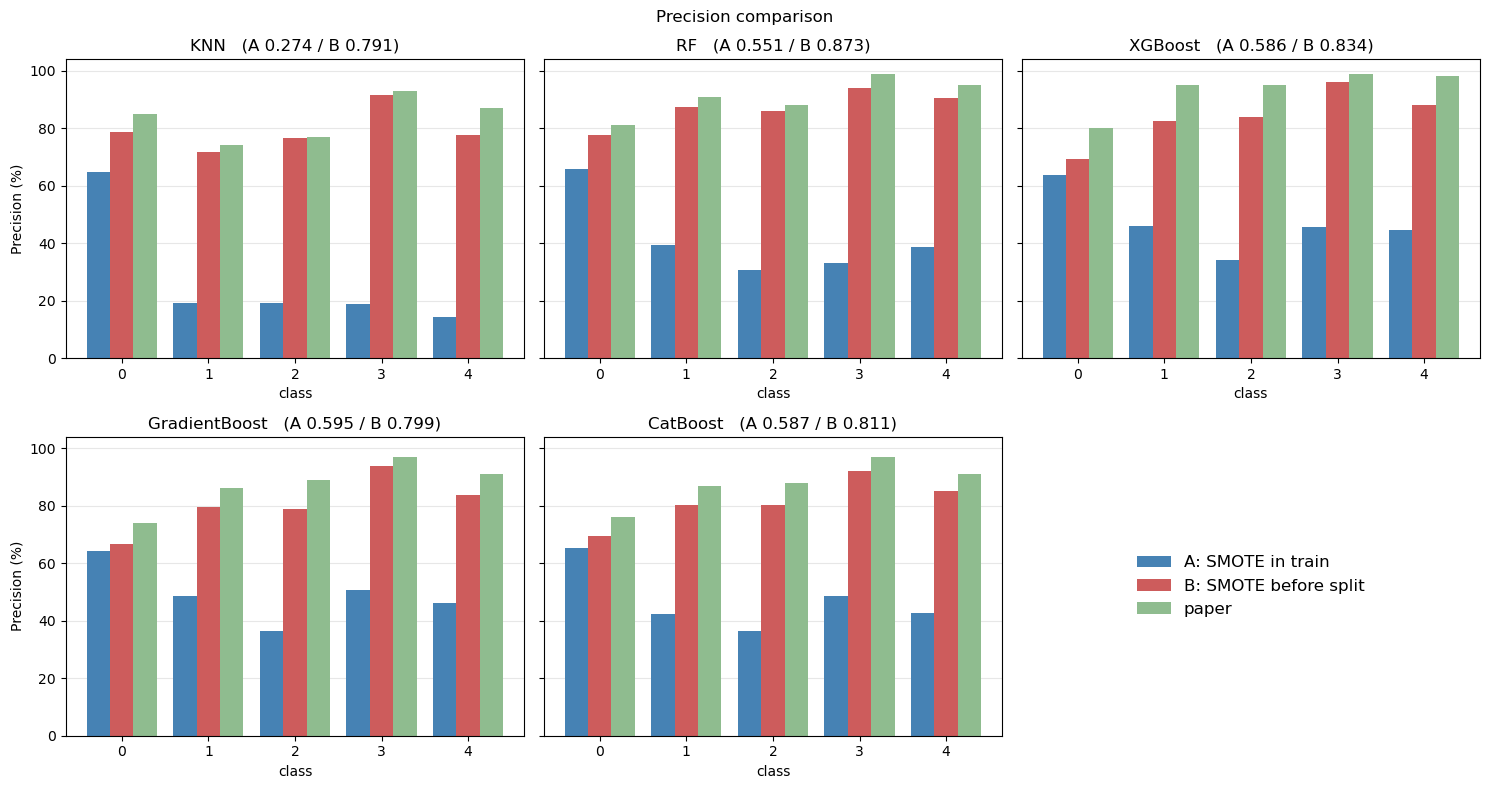
\includegraphics[width=0.9\textwidth]{figures/part1/ablation_precision.png}
\end{figure}

\begin{figure}[H]
    \caption{Comparison on class–wise recall for each model.}
    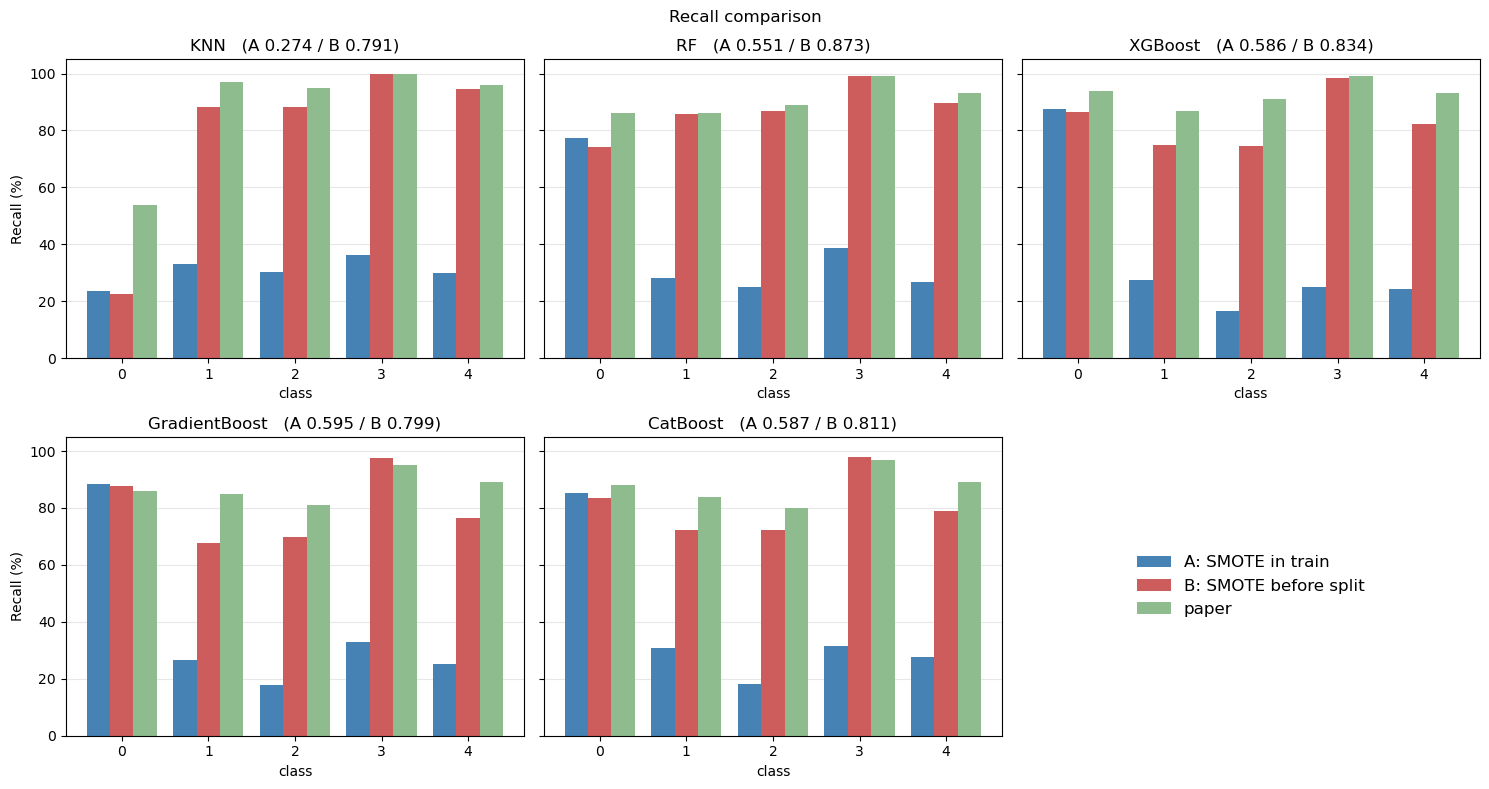
\includegraphics[width=0.9\textwidth]{figures/part1/ablation_recall.png}
\end{figure}

\begin{figure}[H]
    \caption{Comparison on class–wise F1 for each model.}
    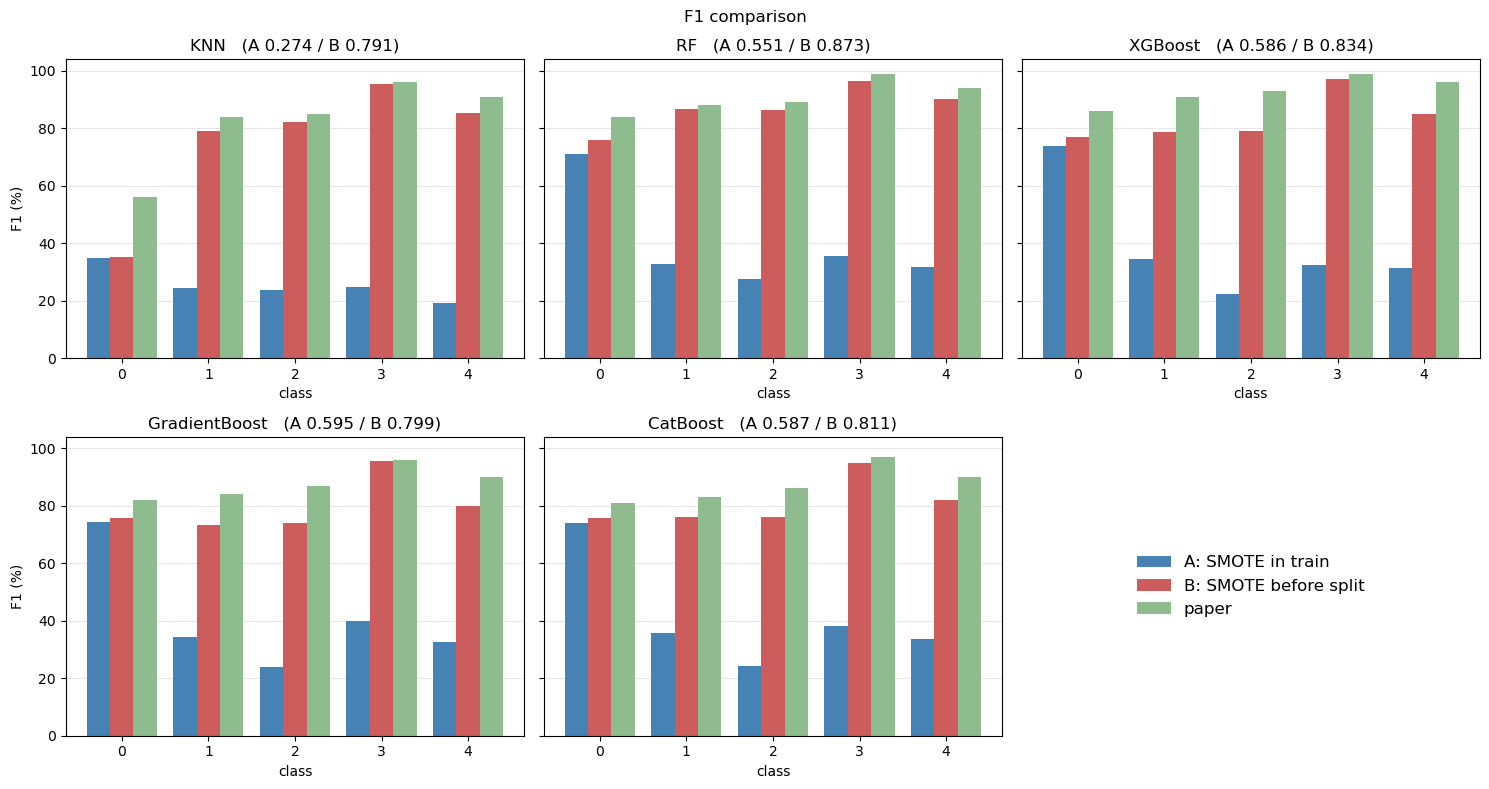
\includegraphics[width=0.9\textwidth]{figures/part1/ablation_f1.png}
\end{figure}

The above–presented bar plots are to aid in the investigation of \textbf{Tab. \ref{tab:cv_classwise_ablation}} visually.
Considering the figures and tables below, although there are moderate deviations from the actual results, we further notice the \textbf{Fig. \ref{fig:ablation_confusion}} and \textbf{Fig. \ref{fig:ablation_roc_curve}} share a very similar patterns.
Interestingly, without further evidence, by changing the flattening strategy, $(12 \times 1000) \to (12000,)$, the gap is much narrower. One can test by switching ``timemajor'' to ``leadmajor'' in \texttt{ablation.ipynb}.

\begin{table}[H]
    \centering
    \caption{\textbf{Protocol B} class–wise performance metrics across models.}
    \label{tab:cv_classwise_ablation}

    \begin{subtable}[t]{0.48\textwidth}
        \centering
        \caption{KNN}
        \label{tab:cv_knn_ablation}
        \begin{tabular}{cccc}
            \toprule
            Class & Precision & Recall & F1 Score \\
            \midrule
            NORM (0) & 81.8 & 23.0 & 35.9 \\
            MI   (1) & 73.4 & 90.8 & 81.2 \\
            STTC (2) & 77.3 & 90.6 & 83.4 \\
            HYP  (3) & 92.4 & 99.9 & 96.0 \\
            CD   (4) & 77.5 & 95.2 & 85.4 \\
            \bottomrule
        \end{tabular}
    \end{subtable}
    \hfill
    \begin{subtable}[t]{0.48\textwidth}
        \centering
        \caption{Random Forest}
        \label{tab:cv_rf_ablation}
        \begin{tabular}{cccc}
            \toprule
            Class & Precision & Recall & F1 Score \\
            \midrule
            NORM (0) & 81.3 & 75.4 & 78.2 \\
            MI   (1) & 88.1 & 87.8 & 87.9 \\
            STTC (2) & 86.7 & 88.7 & 87.7 \\
            HYP  (3) & 94.1 & 99.2 & 96.6 \\
            CD   (4) & 91.0 & 90.8 & 90.9 \\
            \bottomrule
        \end{tabular}
    \end{subtable}

    \bigskip

    \begin{subtable}[t]{0.48\textwidth}
        \centering
        \caption{Histogram–based Gradient Boosting}
        \label{tab:cv_gb_ablation}
        \begin{tabular}{cccc}
            \toprule
            Class & Precision & Recall & F1 Score \\
            \midrule
            NORM (0) & 68.5 & 87.5 & 76.8 \\
            MI   (1) & 79.6 & 69.8 & 74.4 \\
            STTC (2) & 79.1 & 70.6 & 74.6 \\
            HYP  (3) & 93.6 & 97.6 & 95.6 \\
            CD   (4) & 84.5 & 77.0 & 80.5 \\
            \bottomrule
        \end{tabular}
    \end{subtable}
    \hfill
    \begin{subtable}[t]{0.48\textwidth}
        \centering
        \caption{AdaBoost}
        \label{tab:cv_ada_ablation}
        \begin{tabular}{cccc}
            \toprule
            Class & Precision & Recall & F1 Score \\
            \midrule
            NORM (0) & 43.4 & 38.6 & 40.6 \\
            MI   (1) & 32.5 & 32.2 & 32.0 \\
            STTC (2) & 31.5 & 32.3 & 31.6 \\
            HYP  (3) & 58.7 & 71.2 & 64.3 \\
            CD   (4) & 37.5 & 32.1 & 34.4 \\
            \bottomrule
        \end{tabular}
    \end{subtable}

    \bigskip

    \begin{subtable}[t]{0.48\textwidth}
        \centering
        \caption{CatBoost}
        \label{tab:cv_cat_ablation}
        \begin{tabular}{cccc}
            \toprule
            Class & Precision & Recall & F1 Score \\
            \midrule
            NORM (0) & 70.4 & 84.6 & 76.9 \\
            MI   (1) & 81.2 & 73.1 & 76.9 \\
            STTC (2) & 80.3 & 73.3 & 76.6 \\
            HYP  (3) & 92.5 & 98.0 & 95.2 \\
            CD   (4) & 86.2 & 79.8 & 82.8 \\
            \bottomrule
        \end{tabular}
    \end{subtable}
    \hfill
    \begin{subtable}[t]{0.48\textwidth}
        \centering
        \caption{XGBoost}
        \label{tab:cv_xgb_ablation}
        \begin{tabular}{cccc}
            \toprule
            Class & Precision & Recall & F1 Score \\
            \midrule
            NORM (0) & 70.9 & 87.2 & 78.2 \\
            MI   (1) & 84.6 & 76.3 & 80.2 \\
            STTC (2) & 84.3 & 76.2 & 80.0 \\
            HYP  (3) & 96.1 & 98.5 & 97.3 \\
            CD   (4) & 88.3 & 83.0 & 85.5 \\
            \bottomrule
        \end{tabular}
    \end{subtable}
\end{table}



\begin{table}[H]
    \centering
    \caption{\textbf{Protocol B} Performance metrics across all models.}
    \label{tab:single_model_wise_ablation}
    \begin{tabular}{ccccccc}
        \toprule
        Metrics & \texttt{XGBoost} & \texttt{RF} & \texttt{CatBoost} & \texttt{AdaBoost} & \texttt{GBoost} & \texttt{KNN} \\
        \midrule
        Precision & 84.8 & 88.2 & 82.1 & 40.7 & 81.1 & 80.5 \\
        Recall & 84.2 & 88.4 & 81.8 & 41.3 & 80.5 & 79.9 \\
        F1 Score & 84.3 & 88.3 & 81.7 & 40.6 & 80.4 & 76.4 \\
        Accuracy & $84.2$ & $88.4$ & $81.8$ & $41.3$ & $80.5$ & $79.9$ \\
        \bottomrule
    \end{tabular}
\end{table}

\begin{figure}[H]
    \centering
    \caption{\textbf{Protocol A} Confusion matrices of all classifiers.}
    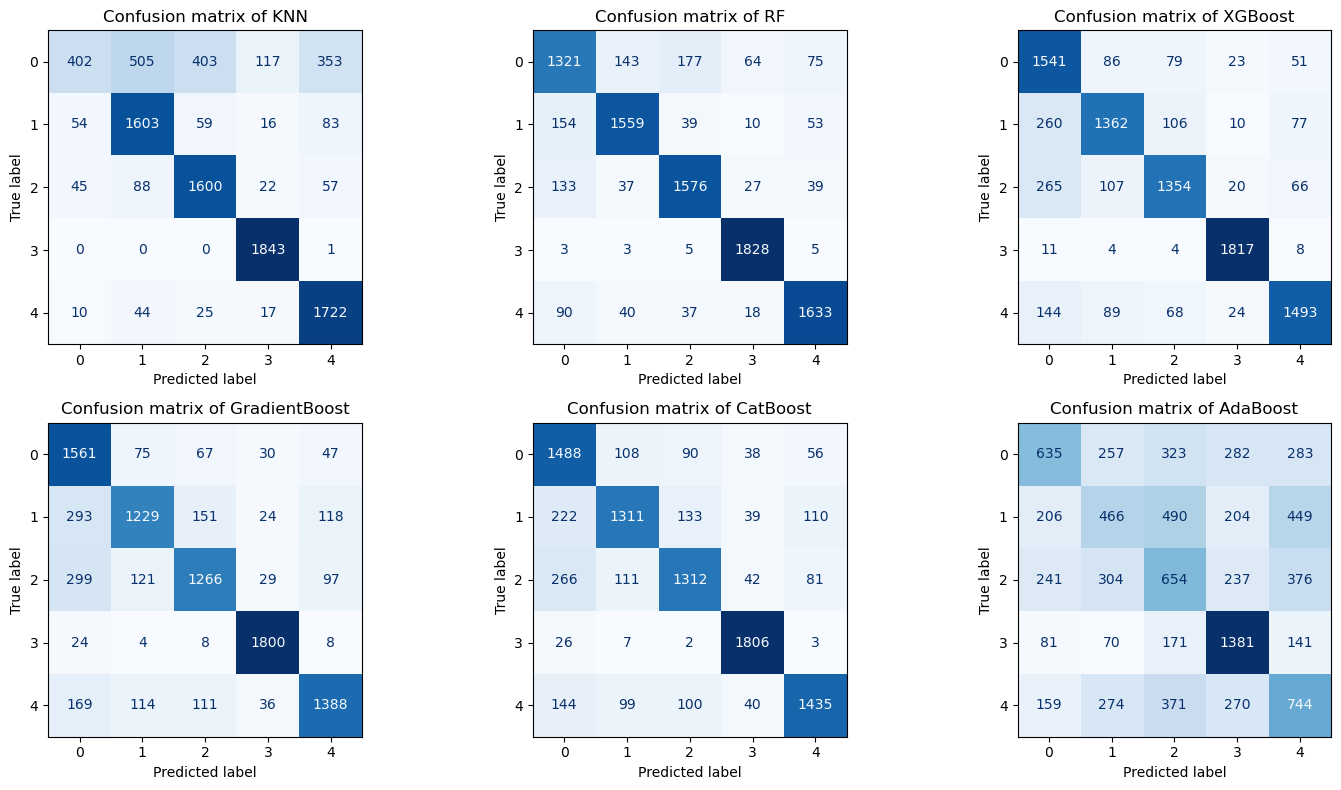
\includegraphics[width=\textwidth]{figures/part1/ablation_confusion.png}
    \label{fig:ablation_confusion}
\end{figure}

\begin{figure}[H]
    \centering
    \caption{\textbf{Protocol A} ROC–AUC curves and scores across classifiers.}
    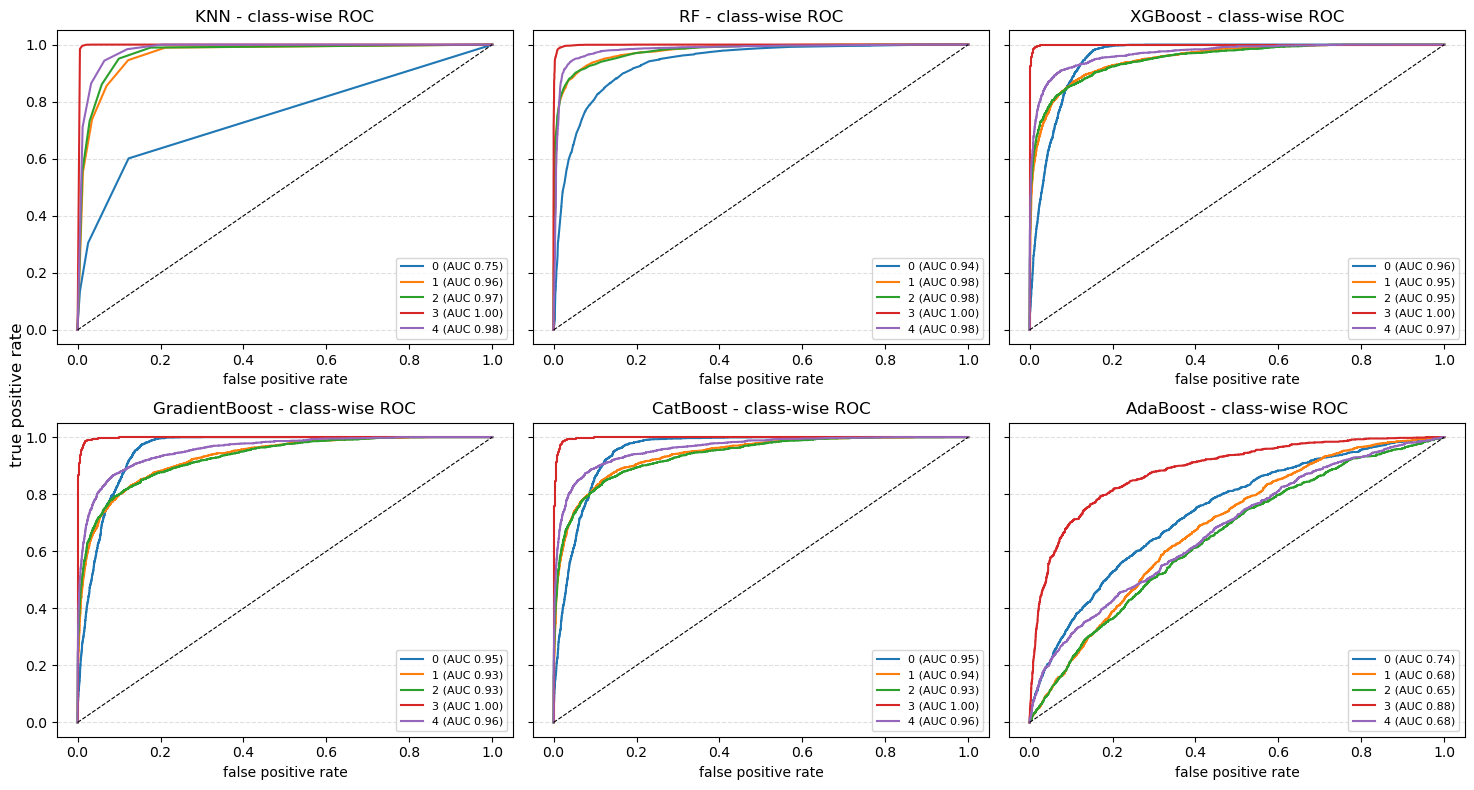
\includegraphics[width=\textwidth]{figures/part1/ablation_roc_curve.png}
    \label{fig:ablation_roc_curve}
\end{figure}

\paragraph{Findings.}
Performing scaling and \texttt{SMOTE} before partitioning takes the ensembles most of the way to the published level.
As the flattening is unchanged from \textbf{Sec. \ref{sec:part_1_method}}, the $39.9$–$49.1$ F1 points the four ensembles gain over \textbf{Tab. \ref{tab:single_model_wise}} are attributable to this leakage alone; \texttt{RF}, for instance, rises from $39.2$ to $88.3$.
The published figures are nevertheless not fully recovered.
All $20$ class–wise F1 scores of \texttt{RF}, \texttt{XGBoost}, \texttt{GBoost} and \texttt{CatBoost} in \textbf{Tab. \ref{tab:cv_classwise_ablation}} fall below the paper's per–class tables \cite{sinha2023dasmcc}, by $0.1$–$13.0$ points, the largest shortfall being STTC under \texttt{XGBoost} ($80.0$ against $93$).
\texttt{RF} comes closest, within $5.8$ points on every class, and replaces \texttt{XGBoost} as the best model; the four ensembles span $80.5$–$88.4\%$ accuracy, against $88.0$–$93.0\%$ in their Table 12.
For the boosted models, NORM precision ($68.5$–$70.9$) lies well below its recall ($84.6$–$87.5$), since \textbf{Fig. \ref{fig:ablation_confusion}} shows minority records absorbed into NORM, e.g. $260$ MI and $265$ STTC records under \texttt{XGBoost}.
\texttt{KNN} still fails on NORM, with F1 $35.9$ against the published $56$, classifying only $402$ of $1{,}780$ NORM records correctly.

Three observations confirm that the leakage reproduces the paper's protocol.
First, recall equals accuracy for all six models in \textbf{Tab. \ref{tab:single_model_wise_ablation}}, which holds only when every class has equal support.
Second, \textbf{Fig. \ref{fig:ablation_confusion}} contains $9{,}069$ test samples spread almost evenly across the classes ($1{,}780$–$1{,}844$ each), mirroring the $9{,}083$ in the paper, whereas a leakage–free $80/20$ split yields $3{,}249$.
Third, HYP, only $3.8\%$ of a leakage–free test split, becomes the easiest class: its F1 is $95.2$–$97.3$ for every model except \texttt{AdaBoost}, and its AUC in \textbf{Fig. \ref{fig:ablation_roc_curve}} reaches $1.00$ for those five models, matching the paper's $1.00$.
